\documentclass[crop,tikz,border=2px]{standalone}
\usepackage{tikzsymbols}
\usetikzlibrary{arrows,positioning,scopes}
\begin{document}
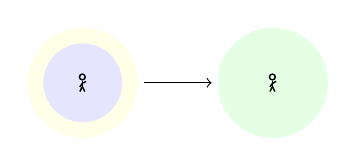
\begin{tikzpicture}[
  ur/.style={circle,minimum width=1.4cm},
  reader/.style={circle,minimum width=1cm,fill=blue!10}]

  \node[ur,fill=yellow!10] (c1) {};
  \node[reader] (c2) {\Strichmaxerl[][54][28]};
  \node[ur,fill=green!10] (c3) [right=of c1] {\Strichmaxerl[][54][28]};

  \draw[->,shorten <=2pt,shorten >=2pt] (c1) -- (c3);
\end{tikzpicture}
\end{document}